\chapter{物理层}\label{CN02}

\par\medskip\noindent\textbf{知识导图}\par\smallskip
\begin{wideblock}\centering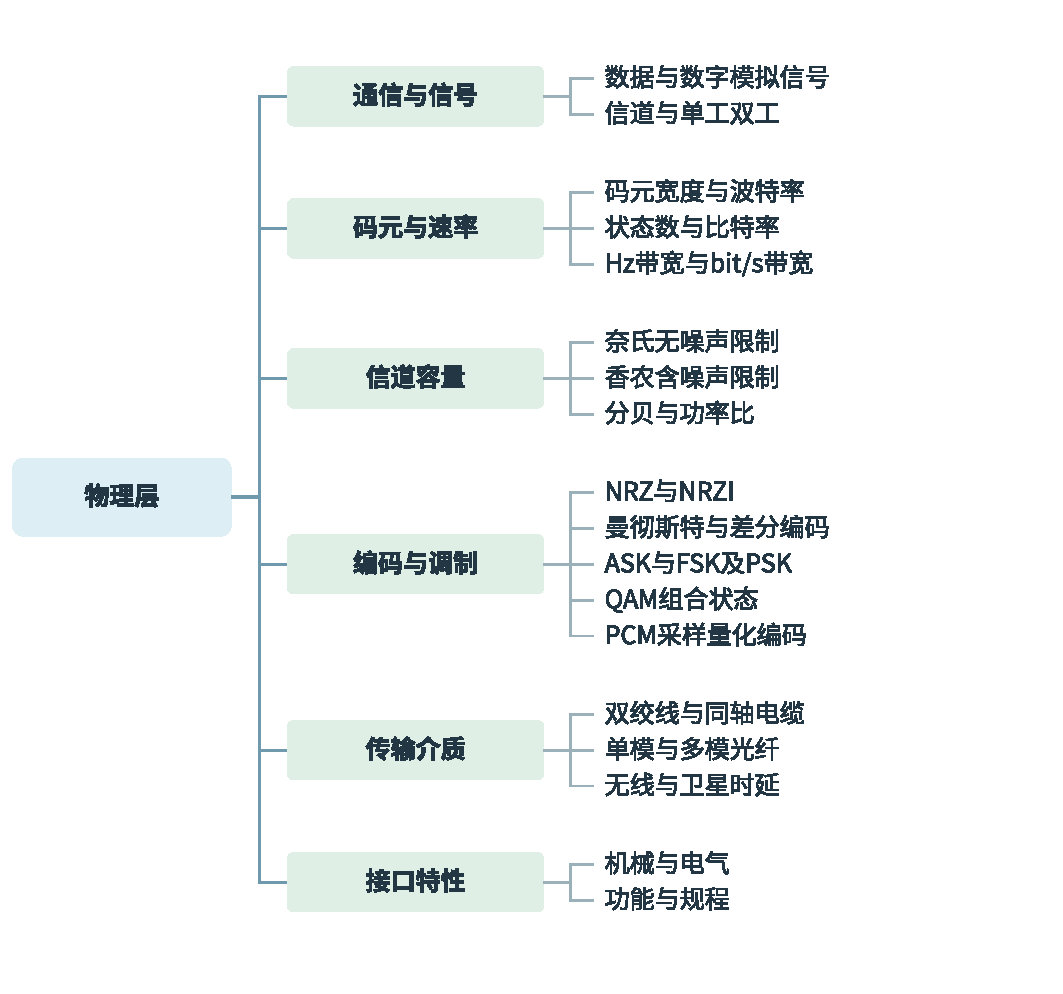
\includegraphics[width=\linewidth,height=168mm,keepaspectratio]{figures/map-01.pdf}\end{wideblock}\par\medskip\clearpage

\par\medskip\noindent\textbf{知识导图（续）}\par\smallskip
\begin{wideblock}\centering
\includegraphics[width=\linewidth,height=168mm,keepaspectratio]{figures/map-02.pdf}\end{wideblock}\par\medskip\clearpage

把``每秒传多少码元''换成``每秒携带多少比特''，必须知道一个码元有多少种状态；把``带宽多大''换成``容量上限''，还要区分带宽单位、噪声与调制约束。本章将这些量放回信号、介质与接口中理解。

\section{数据、信号、码元与两种带宽}\label{CN02-01}

\begin{definition}[数据与信号]

\textbf{数据}承载信息，\textbf{信号}是数据在介质中的物理表示。数字数据可以表示为离散电平，也可以调制在连续载波上；模拟语音可以直接调制传输，也可以采样量化后编码为数字数据。因此不能把``模拟数据''与``模拟信号''当作同一概念。

\end{definition}

\textbf{码元}是在一个固定时间间隔内选取的一种信号波形或状态。若有 \(M\) 种可区分状态，一次可表示 \(\log_2M\) bit；码元速率 \(R_s\) 的单位为 Baud，数据速率 \(R_b\) 的单位为 bit/s。在题目把每个状态按等长二进制编码、忽略其他冗余时，

\[R_b=R_s\log_2M.\]

例如1000 Baud 达到4 kb/s，需要每码元4 bit，即 \(M=2^4=16\) 种状态，不能把4误当成状态数。若题给``每 \(1/8\) s 取一个可独立传送的16态符号''，则速率是 \(8\times4=32\) bit/s；这里8已是每秒符号数，不必再乘2。〖2.1-007〗〖2.1-016〗

\textbf{频率带宽}指可通过频率范围的上、下限之差，单位 Hz；\textbf{数据率意义的带宽}指单位时间能传送的数据量，单位 bit/s。看到``4 kHz信道''应想到容量定理，看到``4 kb/s链路''通常已给出数据传输速率。两者单位不同，数值不能直接互换。

信道是某一方向上传送信号的通道。一条物理线路可以承载多个按频率、时间或编码区分的逻辑信道。单工只能单向传送，半双工可双向但不能同时，全双工可同时双向。两端之间有一根网线，不足以判断它采用哪一种工作方式。

\section{奈奎斯特与香农：哪个条件限制了速率}\label{CN02-02}

理想无噪声低通信道频率带宽为 \(B\) Hz 时，无码间串扰的极限码元速率是 \(2B\) Baud；若每码元有 \(M\) 种状态，奈奎斯特式给出

\[R_b\le 2B\log_2M.\]

带宽限制了可独立辨认的变化速度。把接收端采样次数增加到 \(2B\) 以上，不会自动创造更多独立码元。〖2.1-010〗中的8 kHz、8态信道，即使写``每秒采样24k次''，仍受 \(2\times8000\times3=48\) kb/s 约束。

有加性高斯白噪声的带限信道，香农容量为

\[C=B\log_2(1+S/N).\]

\(S/N\) 是无单位的功率比。若给出分贝数 \(\gamma\)，先计算 \(S/N=10^{\gamma/10}\)。30 dB 对应1000，不能把30直接代入对数。容量是理论上的可靠传输极限：编码合适、码长足够长时，实际速率可以趋近它，但任何具体调制器都不一定达到。

题目同时给出带宽、状态数和信噪比时，通常要检查固定调制状态数与噪声各自施加的限制，再按题目的教材信道模型取较小的上界；两式不是相加关系。若二进制信号在4 kHz、信噪比127的信道上传送，固定二进制给出8 kb/s，而香农给出28 kb/s，能采用的上界为8 kb/s。〖2.1-012〗

\begin{methodbox}[容量题的四步换算]

先把频率带宽换为Hz、分贝换为功率比，再由状态数求每码元比特数；分别计算题设允许的奈氏与香农上界，最后选有效约束。只给码元率时直接乘\(\log_2M\)，不要无依据再乘2。

\end{methodbox}

\begin{wideblock}

\par\medskip\noindent\begin{minipage}{\linewidth}\fontsize{9.3}{12}\selectfont\begin{tabularx}{\linewidth}{@{}YYY@{}}
\toprule\noalign{}
已知信息 & 计算关系 & 条件与单位 \\
\midrule\noalign{}


每秒码元数与状态数 & \(R_b=R_s\log_2M\) & 理想等长编码，不计额外冗余 \\
无噪声低通带宽 & \(R_s\le2B\) & \(B\)用Hz，码元率用Baud \\
带宽与功率比 & \(C=B\log_2(1+S/N)\) & 高斯噪声模型，结果bit/s \\
分贝信噪比 & \(S/N=10^{\gamma/10}\) & 功率比，无单位 \\
\bottomrule\end{tabularx}
\end{minipage}\par\medskip

\end{wideblock}

每个码元有\(M\)种可区分状态，连续\(q\)个码元共有\(M^q\)种序列；若想表示\(k\)位二进制信息，需要至少\(2^k\)种序列，故\(k\le q\log_2M\)。将每秒码元数乘进去，得到理想速率关系。状态数是指数空间，不能把\(M\)直接当每码元比特数。

\subsection{例 2-1　由调制状态数求最大速率}\label{CN02-ex1}

\begin{example}[配套例题]

配套例题。 在一条带宽为200 kHz的无噪声信道上，若采用4个幅值的 ASK 调制，则该信道的最大数据传输速率是（　）。

A. 200 kb/s　B. 400 kb/s　C. 800 kb/s　D. 1600 kb/s

\end{example}

\textbf{解析。} ``无噪声、带宽、4个幅值''分别给出了奈氏模型、\(B=200000\) Hz 和 \(M=4\)。每个码元携带2 bit，极限码元率为400 kBaud，因此最大数据率为800 kb/s，选 \textbf{C}。把200 kHz直接当成200 kb/s，会同时丢掉码元速率与每码元比特数两个转换。

\subsection{例 2-2　增加信噪比是否一定提高固定调制的极限}\label{CN02-ex2}

\begin{example}[配套例题]

〖2.1-017〗 某信道带宽为10 MHz，信噪比为30 dB，采用 QAM-32 调制。若带宽提高到20 MHz，信噪比提高到40 dB，则信道的极限数据传输速率大约提高到原来的（　）倍。

A. 2　B. 2.2　C. 2.4　D. 2.6

\end{example}

\textbf{解析。} QAM-32每码元5 bit。按题设模型，原奈氏上界为100 Mb/s，原香农上界约为 \(10\log_2(1001)=99.67\) Mb/s；新奈氏上界为200 Mb/s，新香农上界约为 \(20\log_2(10001)=265.76\) Mb/s。因此新旧上界的比值约为 \(200/99.67=2.01\)，最接近 \textbf{A}。

原条件下两个上界非常接近，按近似 \(\log_21000\approx10\) 也得到约2倍。新增信噪比使噪声约束放宽，但固定32态调制仍限制每个码元只能携带5 bit，所以不能仅用两个香农容量之比作答。

\section{编码、调制与 PCM 怎样区分}\label{CN02-03}

基带编码用电平及跳变表示数字数据。非归零 NRZ 在一个比特间隔保持某一电平，连续相同比特可能没有跳变，时钟恢复困难。反向非归零 NRZI 用比特起点是否跳变表示数据，具体0、1约定要由题目给出；长串相同比特仍可能缺少跳变，常需填充等机制。

曼彻斯特编码在每个比特中点都跳变，以跳变方向表示数据。本书示意约定低到高为0、高到低为1；题目若采用相反约定，应按题意读图。差分曼彻斯特同样在每个比特中点跳变，但由\textbf{比特起点是否跳变}表示数据，本书约定起点跳变为0、不跳变为1。判断差分编码的第一位需要知道前一电平；不能只看该位中点的升降方向。

\par\medskip\noindent\begin{minipage}{\linewidth}
\centering
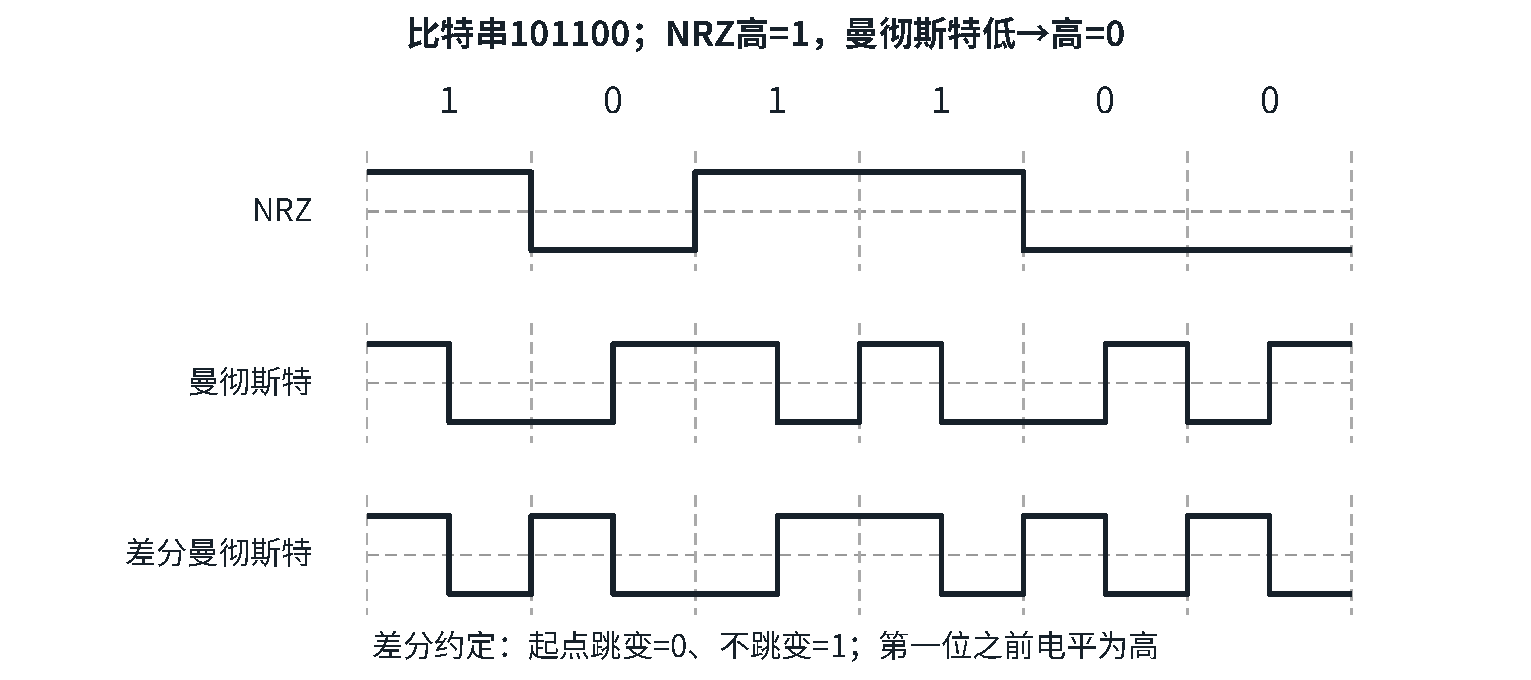
\includegraphics[width=\linewidth,height=125mm,keepaspectratio]{figures/CN03_line_coding.pdf}
\captionof{figure}{同一比特串的三种基带表示；虚线划定比特间隔}\label{cn-fig-coding}
\end{minipage}\par\medskip

曼彻斯特每位需要两个半位信号区间，因此在教材``每秒最多可承载多少电平区间''的模型中，数据率只有该区间变化能力的一半。不要因此认为比特中点的每次跳变都额外携带一位数据；中点跳变还承担时钟作用。

调制把数据映射到载波参数。ASK 改变振幅，FSK 改变频率，PSK 改变相位；QAM 联合使用振幅与相位区分状态。4个相位、每个相位4种振幅共有16态，每码元4 bit。QAM-64表示64种可分辨组合，不是64个比特，也不是64个独立频率。

模拟数据转为数字数据常采用 PCM：先采样取得离散时刻的幅值，再量化为有限级别，最后将级别编码。对最高频率为 \(f_{\max}\) 的理想带限信号，采样频率应不低于 \(2f_{\max}\)；若每样本编码 \(q\) bit，未计信道编码冗余的数据率为 \(f_s q\)。这里的``采样至少两倍''与前节``码元至多两倍带宽''分别限制采样与无码间串扰传输，不能一看到``2''就无条件相乘。

例如电话语音按8 kHz采样、每样本8 bit，产生64 kb/s数据；若再用带冗余的线路编码，物理线路需要承担的编码后速率还会增加。4B/5B用5个线路比特表示4个数据比特，编码效率为4/5；这一效率与每码元的调制阶数是两个不同因素。

\section{传输介质：比较受什么条件约束}\label{CN02-06}

双绞线由两条相互绝缘的导线绞合而成，以减少电磁干扰；屏蔽双绞线进一步增加屏蔽结构。同轴电缆用内导体、绝缘层和外导体屏蔽层构成，传统条件下具有较好的屏蔽性能。介质的实际速率同时取决于编码、设备、频段、长度等条件，不宜一概断言``同轴一定比所有双绞线快''。

光纤利用光信号传播，绝缘且不受外界电磁干扰，衰减较低。多模光纤允许多种传播模式，不同模式到达时间不同，会产生模间色散；单模光纤减轻这类展宽，适用于更长距离和较高容量的通信。多模与单模的区别不只是``同时发送几种颜色''；多种波长复用是另一种复用技术。

无线介质包括无线电、微波、红外等。低频无线电较易绕射，地面微波常要求视距传播，卫星通信能覆盖较大区域，但高轨卫星的长传播距离带来明显时延。不能把光纤``速率高''理解为其中信号的传播速度一定高于无线电波在真空中的速度。

常见以太网名称也需要读出限定：10BASE-T采用双绞线；10BASE5是传统粗同轴、单段上限500 m的制式；100BASE-T主要使用双绞线。500 m不是一切同轴网的共同极限。吉比特以太网不同物理制式使用不同编码，不能沿用传统10 Mb/s以太网的曼彻斯特编码概括全部制式。

\section{物理层接口规定什么，不规定什么}\label{CN02-07}

机械特性规定连接器形状、尺寸及接点排列等；电气特性规定电压、电平、阻抗与传输速率等；功能特性说明各条信号线承担什么功能；规程特性规定信号出现的顺序和双方动作次序。接点``位于哪里''属于机械特性，接点``用来请求发送''属于功能特性，不能都按``引脚''一个词归类。

\subsection{例 2-5　MAC 地址属于物理层接口规范吗}\label{CN02-ex5}

\begin{example}[配套例题]

配套例题。 下列选项中，不属于物理层接口规范定义范畴的是（　）。

A. 接口形状　B. 引脚功能　C. 物理地址　D. 信号电平

\end{example}

\textbf{解析。} 形状、引脚功能和电平分别对应机械、功能与电气特性。这里的``物理地址''指 MAC 地址，是链路层寻址标识，并不因为名称中有``物理''就属于物理层接口规范，选 \textbf{C}。

\section{中继器与集线器：再生比特，不解释地址}\label{CN02-08}

数字中继器在信号衰减、失真后再生符合规范的比特信号，重点是判决、整形和重新发送，不是把噪声和有用信号一起按幅度放大。它不检查 MAC 地址，也不学习转发表或进行网络层路由。可在满足速率、编码和协议等兼容条件时连接不同介质；``能换介质''不等于``能翻译不同网络协议''。

集线器是多端口中继器。一个端口收到比特后向其他端口转送，所有站仍共享一个冲突域、同一份总带宽。5台主机接10 Mb/s集线器，在理想均分且不计竞争开销的模型下每台平均为2 Mb/s；不是每台始终保证2 Mb/s，也不是五台主机可以同时各以10 Mb/s发送。

一个集线器两侧各100 m、传播速率 \(2\times10^8\) m/s 时，最远站点间单向路径为200 m，传播1 μs，往返2 μs。〖3.6-020〗的计算先合计两侧距离，再考虑往返；只把100 m乘2得到单向路径就停下，会漏掉回程那一段。中继设备若有额外时延也应计入，不能只看电缆长度。

\section{主动回忆自测}\label{CN02-review}

以下为自拟题，先标出单位和模型条件再作答。

\begin{enumerate}
\def\labelenumi{\arabic{enumi}.}
\tightlist
\item
  每秒2000个码元、每码元8态，忽略冗余，数据率是多少？改为16态而码元率不变呢？
\item
  频率带宽1 MHz、信噪比30 dB，香农式应代入30还是1000？
\item
  2 kHz无噪声低通信道采用16态，理想最大码元率和比特率分别为多少？
\item
  曼彻斯特的中点跳变与差分曼彻斯特的起点跳变各表示什么？
\item
  最高频率4 kHz的带限模拟信号每次采样编码8 bit，按最低理想采样率得到多少bit/s？
\item
  连接器形状、某引脚用于请求发送、信号电平和信号出现次序分别属于哪类接口特性？
\item
  五台主机连接10 Mb/s集线器，是否能同时各发10 Mb/s？
\item
  光纤提高传输容量，是否必然使同距离上的传播时延比真空无线传播更短？
\end{enumerate}

\subsection{核对答案}\label{CN02-review-answers}

\begin{enumerate}
\def\labelenumi{\arabic{enumi}.}
\tightlist
\item
  分别6 kb/s和8 kb/s，按码元率乘每码元信息量。
\item
  1000，容量为\(10^6\log_2(1001)\) bit/s。
\item
  4000 Baud与16 kb/s；必须保留题设低通无噪声模型。
\item
  曼彻斯特中点跳变承担同步并由方向表意；差分曼彻斯特中点仍用于同步，起点是否跳变表意，具体0/1约定按题目。
\item
  最低理想采样8000次/s，所得64 kb/s，未计其他冗余。
\item
  依次为机械、功能、电气、规程特性。
\item
  不能，它们共享总带宽和冲突域；理想均分2 Mb/s只是特定平均模型。
\item
  不必然，容量与传播速度是不同量；传播时延仍按介质中的速度和距离计算。
\end{enumerate}
